%%% Inicio del documento se define la clase y
%%%tesisupiita )Tesis: UPIITA-IPN
%Copyright (C) 2017 Juan Carlos Guzm�n Salgado
%% Griselda S�nchez Otero
%%% propiedades generales
\documentclass[letterpaper,11pt]{upiita}
%%%%%%%%%%%%%%%%%%%%%%%%%%%%%%%%%%%%%%%%%%%%%%%%%%%%%%%%%%%%%%%%%%%%%%%
%%%%%%%%%%%%%%%%%%%%%%%%%%%%%%%%%%%%%%%%%%%%%%%%%%%%%%%%%%%%%%%%%%%%%%%
%%%%%%%%%Paquetes utilizados%%%%%%%%%%%%%%%%%%%%%%%%%%%%%%%
%%%%%%%%%%%%%%%%%%%%%%%%%%%%%%%%%%%%%%%
\usepackage{upiitatesis}
\usepackage{float}
\usepackage{makeidx}
\usepackage{amsfonts}
\usepackage{amsmath}
\usepackage{mathrsfs}
\usepackage{eucal}
\usepackage{mathrsfs}
\usepackage{graphicx}
\usepackage{lettrine}
\usepackage[pdftex=false,colorlinks=true]{hyperref}
\usepackage[spanish]{babel}
\usepackage[latin1]{inputenc}
\usepackage[Sonny]{fncychap}
\usepackage{fancyhdr}
\usepackage{subfigure}
\usepackage{layout}
\usepackage{textcomp}
\usepackage{bbding}
\usepackage{ifthen}
\usepackage{pifont}
\usepackage{romanidx}
\usepackage{titlesec}
\usepackage{titling}
%%Propiedades adicionales
%%%%%%%%%genera secci�n de �ndice %%%%%%%%%
\makeindex
%%%%%%%%%%%%%%%%%%%%%%%%%%%%%Inicio de documento}}}
\begin{document}
%%%%%%%% Inicio de Secci�n de preliminares numeraci�n con n�meros romanos%%%%
\frontmatter
%%%%%%%%%%%%%  Datos de la Portada y acta
\title{Rodamientos Magn�ticos H�bridos}
\unidad{\Upiita}
\materia{Trabajo Terminal II}
\academia{Mecatr\'onica}
\degree{Ingeniero en Mecatr\'onica}     %%%%%%%%%%%%%grado
\degreemonth{MAYO}                     %%%%%%%%%%mes
\degreeyear{2017}                       %%%%%%%%%%a�o
%%%%%%%%%%%%  Nombre del Presidente y Secretario del jurado
\Presidente{M. en C. Alfonso Campos V�zquez}
\Titular{M.en C. Griselda S�nchez Otero}
%%%%%%%%%%%%%%%%%%%%%%% Datos del autor%%%%%%%%%%%
%%%%%%%%%%%%%%%%%%%%%%%%%%%%%%%%%%%%%%%%%%%%%%%%%
%%para varios asesores (m�ximo 4) y autores (alumnos) dejar el campo en blanco de los que no deban aparecer
%%%%%%%%%% Cuando el n�mero de asesores=1 s�lo se toma en cuenta la variable alumnoa,
%%                                     =2 se toman alumnoa y asesorb, etc
%%%%%%%%%%%%%%%%%%%%%%%%%%%%%
\nalumnos{3}
%%%%%%% dependiendo del numero de alumno dejar vac�o el campo de alumnoX, nunca eliminar o comentar la l�nea
\alumnoa{Omar Alejandro Bejarano Montiel}
\alumnob{Oscar Enriquez Ramirez}
\alumnoc{Manuel Enrique Limones Urbina}
%\alumnod{Giovanni Karol}
%%%%%%%%%% n�mero de asesores 1= solo se toma en cuenta la variable asesora, 2= se toman asesora y asesorb
\nasesores{1}
%%%%%%% en caso de un �nico asesor dejar vac�o el campo de asesorb, nunca eliminar o comentar la l�nea
\asesora{M. en C. �lvaro Gordillo Sol}
%\asesorb{Dr. Johannes Carolus}
%\asesorc{Dr. Ivan Karurosu}
%%creacion de p�ginas
\portada
\acta
\dedicatoria              %%%modificar archivo dedica.tex
\agradecimientos          %%%modificar archivo agradece.tex
\tableofcontents
\listoffigures
\listoftables
\chapter{Resumen}

\textbf{\Large Rodamientos Magn�ticos H�bridos}\\



\textbf{Palabras Clave:} ... \\

\textbf{Resumen:}

...

\textbf{Abstract:}

...
               %%%modificar archivo Resumen.tex
\chapter{Nomenclatura}

lista de nomenclaturas          %%%modificar archivo Nomenclatura.tex
\chapter{Simbolog\'ia}


Simbolo1             %%%modificar archivo Simbologia.tex
\chapter{Objetivos}

\section*{Objetivo general}
Dise�ar y simular un sistema de rodamientos magn�ticos capaz de operar en condiciones de carga est�tica.

\section*{Objetivos Particulares.}

{\setlength{\parindent}{0pt}Trabajo Terminal I:}
\begin{enumerate}
\addtolength{\itemsep}{0pt}
\item Obtener el dise�o conceptual del rodamiento magn�tico h�brido.
\item Obtener el dise�o conceptual del rodamiento magn�tico h�brido.
\item Seleccionar el material ferromagn�tico para el n�cleo de los electroim�nes. 
\item Calcular la secci�n transversal de los electroim�nes.
\item Obtener la geometr�a y dimensiones de los rodamientos activos radial y axial.
\item Validar el punto de operaci�n del electroim�n mediante simulaci�n.
\item Dise�ar un electrodo de alta sensitividad para el rango de operaci�n.
\item Dise�ar un dispositivo para la retracci�n del im�n permanente. 
\item Proponer un circuito de adquisici�n y control. 
\end{enumerate}
\hfill \break

{\setlength{\parindent}{0pt}Trabajo Terminal II:}
\begin{enumerate}
\addtolength{\itemsep}{0pt}
\item Obtener un modelo de electroim�nes que integre los efectos del flujo marginal.
\item Realizar las simulaciones de la fuerza magn�tica ejercida por los electroim�nes y el im�n permanente.
\item Obtener el modelo din�mico del sistema.  
\item Comparar algunos esquemas de control para la estabilizaci�n del sistema.
\item Dise�o del circuito de potencia de los electroim�nes. 
\item Estimar los l�mites de operaci�n del rodamiento con base en las simulaciones.
\end{enumerate}             %%%modificar archivo objetivos.tex
%%%%General
%%%%Espec�ficos
\chapter{Introducci\'on}

El desarrollo de nuevas investigaciones y nuevas tecnolog�as han permitido que la industria busque nuevas y mejores formas de llevar a cabo sus procesos productivos, lo que requiere, entre otras cosas, de transformar y actualizar la maquinaria y equipo que utilizan con el prop�sito de volverlos m�s eficientes y aumentar su productividad.
En este aspecto se han realizado numerosos avances y descubrimientos, como pueden ser el uso de fuentes de energ�a m�s limpias y eficientes, la implementaci�n de nuevos materiales m�s ligeros y resistentes, y por supuesto el reemplazo de algunos componentes y dispositivos por otros m�s avanzados.
Gran parte de la maquinaria industrial posee elementos de tipo rotativo, los cuales requieren el uso de dispositivos denominados cojinetes, tambi�n conocidos como rodamientos o baleros. Estos suelen situarse entre dos componentes de la maquina con un eje de rotaci�n com�n, facilitando el movimiento de giro de un componente con respecto al otro y reduciendo la fricci�n de los diferentes elementos m�viles; son a su vez, un punto de apoyo para dichos ejes o �rboles. 
Adem�s de ser capaces de disminuir la fricci�n, de manera general los rodamientos deben cumplir con algunas caracter�sticas particulares, como son: disminuir las vibraciones, operar de manera silenciosa y poseer una prolongada vida �til. Sin embargo, los distintos sectores industriales suelen establecer sus propios requisitos espec�ficos con base en determinados entornos operativos o aplicaciones particulares, entre los que podemos mencionar: resistir grandes cambios de temperatura, humedad, suciedad, operar en medios agresivos como soluciones acidas o alcalinas, soportar altas velocidades e incluso ser aptos para el contacto con alimentos.
Es por ello que dentro de los rodamientos existe una gran variedad de configuraciones, materiales y modos de operaci�n que puedan satisfacer esta demanda de necesidades.


\section*{Clasificaci�n de Cojinetes y Rodamientos}
%\label{sec:intro:address}
%\addcontentsline{toc}{section}{Clasificaci�n de Cojinetes y Rodamientos}

Los cojinetes se clasifican principalmente en dos grandes grupos: cojinetes de deslizamiento (o de fricci�n) y antifricci�n (rodamientos). Los cojinetes de deslizamiento consisten b�sicamente en un par de casquillos conc�ntricos que giran en contacto directo uno con el otro realiz�ndose un deslizamiento por fricci�n, procurando que esta sea la menor posible; la disminuci�n de la fricci�n depende de los materiales con los que est�n fabricados y del uso de alguna pel�cula lubricante [2]. 
Por su parte, los cojinetes antifricci�n (rodamientos) comprenden una clasificaci�n m�s extensa debido a su complejidad estructural, en comparaci�n a los cojinetes de deslizamiento. Entre los principales podemos encontrar: por la direcci�n de la carga que soportan (axial, radial, angular o mixta, y lineal), seg�n su rigidez (r�gidos y pivotantes) y por el tipo de cuerpo rodante (de bolas, rodillos, agujas, c�nicos, etc.) [3]. 
El rozamiento por rodadura generado por los rodamientos es mucho menor que el de los cojinetes de deslizamiento, y es por ello que presentan una serie de ventajas m�s frente a la utilizaci�n de casquillos que incluye mayor velocidad admisible, menor temperatura de funcionamiento, mayor capacidad de carga, menor desgaste, facilidad de recambio y disminuci�n en los costos de mantenimiento. 
A pesar de todo esto, existen algunas aplicaciones para las cuales se deben buscar alternativas a estos dispositivos mec�nicos, particularmente las que est�n relacionadas con m�quinas rotativas de alta velocidad donde se incrementan de manera considerable las perdidas mec�nicas, las cuales est�n asociadas al rozamiento y a las vibraciones mec�nicas. Ante este problema surge un tipo de rodamiento que opera por medio de la suspensi�n magn�tica, conocidos como rodamientos magn�ticos.  

\section*{Rodamientos Magn�ticos}
%\label{sec:intro:motivation}
%\addcontentsline{toc}{section}{Rodamientos Magn�ticos}

Como ya se mencion� anteriormente, los rodamientos magn�ticos son una excelente alternativa para su uso en m�quinas rotativas de alta velocidad, ya que presentan m�ltiples ventajas frente a los rodamientos tradicionales, como una mayor velocidad de giro, no requieren de un sistema de lubricaci�n ya que operan sin contacto, por lo que adem�s no producen part�culas de desgaste y debido a su baja rigidez son capaces de compensar las vibraciones mec�nicas, haci�ndolos silenciosos. Todo esto se traduce en una disminuci�n de los costos de mantenimiento y prolongaci�n de la vida �til del sistema. 
El potencial que poseen para generar muy pocas p�rdidas y alcanzar mayores velocidades los hace ideales para aplicaciones industriales como centrifugadoras de alta velocidad, volantes inerciales, compresores y turbinas de alto r�gimen de revoluciones, por mencionar algunas. 
Los rodamientos magn�ticos cuentan, a su vez, con una clasificaci�n que viene en funci�n de dos principales factores: de acuerdo a la naturaleza de su fuerza, que puede ser de Reluctancia o de Fuerza de Lorentz, o m�s com�nmente de acuerdo a la fuente generadora del campo magn�tico (Pasivos, Activos e H�bridos) [4]. 
Los pasivos carecen de alimentaci�n externa y emplean imanes permanentes para generar los campos magn�ticos de levitaci�n, mientras que los activos utilizan electroimanes y requieren de una fuente de alimentaci�n externa y de un sistema de control. Por su parte, los h�bridos emplean imanes permanentes para crear un campo base de levitaci�n mientras que el resto del campo es generado por electroimanes.
A pesar de que la mayor�a de los usos que se le dan a los rodamientos magn�ticos pertenecen al sector aeroespacial, naval, generador de energ�a y otras aplicaciones de alta demanda, tambi�n es posible aprovecharlos en otro tipo de maquinaria m�s comercial pudiendo explotar al m�ximo sus beneficios. 


\section*{Antecedentes}
\subsection*{Investigaci�n y Desarrollo de Rodamientos Magn�ticos}
%\label{sec:intro:results}
%\addcontentsline{toc}{section}{Antecedentes}
%\addcontentsline{toc}{subsection}{Investigaci�n y Desarrollo de Rodamientos Magn�ticos}

Investigaci�n y Desarrollo de Rodamientos Magn�ticos 
A pesar de las m�ltiples ventajas que presentan, los rodamientos magn�ticos no est�n exentos de algunos problemas que pueden dificultar su desarrollo e implementaci�n en los sistemas industriales, entre los que podemos destacar el alto consumo energ�tico que generan.
Ante este problema se hicieron varias investigaciones cuyas soluciones pueden clasificarse en dos tipos: el dise�o de algoritmos para minimizar las corrientes en los electroimanes y el uso de imanes permanentes para proveer un campo magn�tico base para la levitaci�n.
La investigaci�n realizada en [5] se trata de una validaci�n experimental en donde 1) se dise�a y construye un prototipo de pruebas que emula el comportamiento de un rodamiento magn�tico activo de un grado de libertad, y 2) se realizaron pruebas para evaluar el desempe�o del controlador inteligente en comparaci�n con un controlador est�ndar de polarizaci�n fija.
Este equipo consiste en un eje r�gido capaz de balancearse libremente sobre un punto de apoyo colocado debajo de su centro de masa. La posici�n angular de este eje es controlada mediante electroimanes fijados a los extremos de este. A pesar su simplicidad este equipo incorpora todas las no linealidades t�picas de un rodamiento magn�tico activo, y la din�mica del sistema es ideal para evaluar el desempe�o de los controladores. 
En [6] una estrategia de control de corriente de polarizaci�n variable es presentada con el fin de minimizar la energ�a consumida sin alterar el desempe�o din�mico del sistema. El modelado parte de un RMA de 2 polos sobre el cual se propone un controlador lineal y un observador de estados para la estimaci�n de estados.
Una vez obtenido el modelo del sistema se calcula de manera anal�tica la corriente �ptima para la estabilizaci�n del sistema y obtener el controlador. 

Como resultado este controlador propuesto fue capaz de reducir el consumo en un 73\%, se estabiliz� la posici�n de rotor en el centro del rodamiento con un error de estado estable nulo y se presentaron vibraciones 60\% menores comparadas con un controlador de polarizaci�n fija.

\subsection*{Rodamientos Magn�ticos en la Industria}
%\label{sec:intro:results}
%\addcontentsline{toc}{subsection}{Rodamientos Magn�ticos en la Industria}

En la actualidad los sistemas de rodamientos magn�ticos tienen m�ltiples aplicaciones dentro del campo industrial, y aunque la mayor�a cuenta con adaptaciones acorde a la maquinaria en la que se utilizar�, poseen una arquitectura y un modo de funcionamiento similar.
La empresa FAG�, filial de Schaeffler Group, ha desarrollado un sistema de rodamiento magn�tico activo que denominan como modular. Su sistema de control y de electr�nica de potencia es capaz de ajustarse a ciertos par�metros definidos por el usuario acorde a los requerimientos de operaci�n, y su dise�o permite una f�cil integraci�n en la arquitectura de la m�quina.
Otra de las ventajas que posee es que pr�cticamente no existen restricciones de velocidad y puede soportar pesos de eje de m�s de 9 toneladas. Cuenta con un sistema de apagado de seguridad que previene da�os a la m�quina y gracias a los cojinetes de respaldo que integra tambi�n la protege en caso de una interrupci�n en el suministro de energ�a que conduzca al fallo del cojinete magn�tico. A su vez sirven de apoyo para el rotor cuando los cojinetes magn�ticos est�n apagados [7].
Sin embargo, ya que se trata de una empresa especializada este producto resulta altamente costoso, adem�s de que �nicamente est�n orientados a aplicaciones de alta demanda y cargas muy grandes.
Por su parte la empresa YORK� Navy Systems de Johnson Controls, quien desarroll� uno de los primeros sistemas de rodamientos magn�ticos para su uso en enfriadores centr�fugos en embarcaciones de grado militar, ha sido capaz de aplicar esta tecnolog�a en enfriadores comerciales, logrando alargar el tiempo de vida de la m�quina disminuyendo el n�mero de partes m�viles y removiendo los sistemas de lubricaci�n tradicionales. Esto se traduce en una reducci�n significativa de los costos de mantenimiento.
Utiliza un sistema de velocidad variable el cual ralentiza el motor cuando el enfriador est� funcionando en condiciones fuera de dise�o, adem�s de mejorar la fiabilidad durante el arranque al asegurar que la corriente de entrada nunca supere el 100% de los amperes de carga completa. Y finalmente gracias a las vibraciones casi indetectables, el ruido se reduce casi por completo [8].
Aunque han logrado ampliar esta tecnolog�a para aplicaciones comerciales e industriales fuero del �mbito militar, este sistema est� desarrollado casi exclusivamente para plantas de enfriamiento y aire acondicionado, por lo que no es capaz de usarse y adaptarse a otro tipo de sistemas.
Por otro lado, la empresa Synchrony� ha realizado grandes avances en cuanto a tecnolog�a de rodamientos magn�ticos se refiere. Han logrado disminuir el tama�o de la unidad de control eliminando o miniaturizado algunos componentes como los convertidores A/D y D/A, los amplificadores de potencia y la interfaz de comunicaciones, y el uso de contadores de alta velocidad para la se�al de posici�n. Una de las innovaciones m�s importantes ha sido el desarrollo de sensores de posici�n que pueden ser integrados directamente en los electroimanes.
Han reducido dram�ticamente el tama�o de los rodamientos magn�ticos axiales y radiales mediante el uso de nuevas e innovadoras t�cnicas de dise�o y manufactura. Todas estas modificaciones han reducido en general la complejidad del sistema [9].
Sin embargo, la disponibilidad de productos es baja, y solamente ofrecen servicio a un n�mero muy limitado de pa�ses.

\section*{Planteamiento del problema}
%\label{sec:intro:results}
%\addcontentsline{toc}{section}{Planteamiento del problema}

En la actualidad, los avances tecnol�gicos tienden hacia el desarrollo de sistemas m�s peque�os, veloces, eficientes, y con un menor consumo de energ�a y m�nimo mantenimiento. Estas cualidades adquieren gran importancia dentro del �mbito industrial, donde sus beneficios impactan directamente en el desarrollo de mejores m�quinas y dispositivos, como motores, compresores, enfriadores, sistemas de centrifugaci�n y sistemas de transmisi�n, por mencionar algunos.
Gran parte de estos y otros dispositivos rotativos no son capaces de alcanzar altas velocidades debido al rozamiento y a las vibraciones que se producen en los ejes y �rboles de transmisi�n; entre m�s revoluciones alcance, mayor ser� el calor generado por la fricci�n, y las p�rdidas mec�nicas incrementan de manera considerable. 
Pese a que los rodamientos suprimen algunas de las desventajas propias de los cojinetes de deslizamiento, a�n presentan algunos inconvenientes para su uso en maquinaria de alta velocidad; estos problemas abarcan principalmente su sensibilidad a la contaminaci�n debido a la generaci�n de part�culas de desgaste, una baja resistencia a las cargas de impacto , generaci�n de cargas fluctuantes  (vibraciones), mayor nivel de ruido ac�stico, y aunque el coeficiente de rozamiento es bajo, los materiales contin�an funcionando en contacto directo, lo que provoca un incremento en las temperaturas de operaci�n. 
Para hacer frente a estas desventajas es necesario considerar el uso de un nuevo tipo de rodamientos que reemplace a los convencionales, por lo que un sistema de rodamientos magn�ticos resulta en una buena alternativa que atrae importantes beneficios. 
Dado que los rodamientos magn�ticos trabajan sin contacto directo con los elementos que soportan, pueden disminuir de manera considerable las p�rdidas mec�nicas debido a la supresi�n del rozamiento de los cojinetes de apoyo y otras partes m�viles. Esto permite reducir la potencia necesaria de los motores e incrementar la eficiencia, y son capaces de compensar las vibraciones y cargas fluctuantes. 
La reducci�n de las p�rdidas implica tambi�n que las temperaturas de operaci�n sean menores, y en algunos casos esto permite que no sea necesario el uso de equipos de refrigeraci�n adicionales. 
Los rodamientos magn�ticos no requieren del uso de lubricantes, lo que los hace ideales para m�quinas que trabajan en ambientes con temperaturas extremas, en condiciones de vac�o, que se encuentren en contacto con sustancias corrosivas o cualquier m�quina que no tolere la contaminaci�n por las part�culas de desgaste o de los mismos lubricantes, adem�s elimina la necesidad de implementar sistemas de lubricaci�n extras.
Todos estos beneficios implican una reducci�n significativa de los costos inherentes al mantenimiento, relacionados principalmente al reemplazo de piezas debido al desgaste, adem�s de la eliminaci�n de sistemas adicionales de refrigeraci�n y lubricaci�n y a una necesidad de mantenimiento peri�dico menor [10]. 
A pesar de las m�ltiples ventajas que ofrece este tipo de sistemas, no se ha logrado ampliar su uso dentro de la industria debido principalmente a que presentan otro tipo de desventajas que no se encuentran en los cojinetes y rodamientos, como su accesibilidad limitada, un precio m�s elevado, la necesidad de contar con un sistema de control y la posibilidad de fallas en el sistema el�ctrico, adem�s de que en el caso de los rodamientos magn�ticos activos el consumo el�ctrico suele ser elevado. Es por eso que en este sentido se opt� por el desarrollo de rodamientos magn�ticos de funcionamiento h�brido, ya que al utilizar un campo base otorgado por los imanes permanentes, el consumo el�ctrico de los electroimanes es menor. 
Este proyecto tendr� como finalidad desarrollar un sistema que pueda brindar una alternativa a los rodamientos magn�ticos tradicionales en proyectos relacionados con el desarrollo de maquinaria y equipo industrial.


\section*{Descripci�n de los Cap�tulos}
%\label{sec:intro:structure}
%\addcontentsline{toc}{section}{Descripci�n de los Cap�tulos}
          %%%modificar archivo introduccion.tex
%%%%%ntecedentes
%%%%%Planteamiento del problema
%%%%%Descripci�n de los cap�tulos
%%%%%%%%%%%%%%%%%%%%%%%%%%%%%%%%%%%%%%%%%
%%%%%%%%%%%%%%%%%%%%%%Inicia Contenido del trabajo%%%%%%%%%%%%%%%%%%%%%%%%%
\mainmatter %\pagenumbering{arabic}
\pagestyle{fancy}
\renewcommand{\chaptermark}[1]{\markboth{#1}{}}
\renewcommand{\sectionmark}[1]{\markright{#1}}
\fancyhf{}
\fancyhead[RO]{\leftmark}
\fancyhead[LE]{\rightmark}
\fancyhead[LO,RE]{}
\fancyfoot{}
\fancyfoot[RO,LE]{\thepage}
\fancyfoot[CO]{UPIITA}
\fancyfoot[CE]{IPN}
\fancyfoot[RE,LO]{Ing. Mecatr�nica}
%%%%%%%%%%%%%%%%%%%%%%%%%%%%%%%%%%%%%%%%%%%%%%%%%%%%%%%%%%%%%%%%%%%
%%%%%%%%%%%%%%%%%%%%%%%%%%%%%%%%%%%%%%%%%%%%%%%%%%%%%%%%%%%%%%%%%%%
%%%%%%%%%%%%%%%%%%%%%%%%%%%%%%%%%%%%%%%%%%%%%%%%%%%%%%%%%%%%%%%%%%%
%%%%%%%%%%%%%%%%%%%%%%%%%%capitulo1111111111%%%%%%%%%%%%%%%%%%%%%%%
\include{Metodologia}
%%%%%%%%%%%%%%CCCCCCCCCCCCCCCCCCCCCCCCCCCCCCCCCCCCC%%%%%%%%%%%%%%%%
%%%%%%%%%%%%%%2222222222222222222222222222222222222%%%%%%%%%%%%%%%%
%\chapter{Dise\~no Conceptual}

\section{Necesidades}

\section{Requerimientos}

\section{Descomposici\'on por funciones}

\section{An\'alisis Morfol\'ogico}

\section{Soluci\'on Dise\~no Conceptual}

\section{Concepto Final}

%\include{disenconcep}
\chapter{Dise\~no Conceptual}

\section{Necesidad}

Los ejes de transmisi�n de las m�quinas se encuentran sometidos constantemente a la fricci�n y a las vibraciones producto del contacto que existe entre estos y las piezas a las que est�n conectados. Esto conlleva una serie de problemas como el aumento de la temperatura de operaci�n y el desgaste de las piezas. Para disminuir estos efectos es necesaria la utilizaci�n de cojinetes o rodamientos sobre los que se sostengan y giren los ejes de transmisi�n.  

Algunas de estas m�quinas requieren operar a un alto r�gimen de revoluciones, y para ello se han desarrollado los rodamientos magn�ticos, los cuales generan un campo magn�tico que ayuda al eje de transmisi�n a permanecer en un estado de levitaci�n, suprimiendo el contacto directo que tendr�a con un cojinete o rodamiento convencional y facilitando el giro del eje. Esto implica una disminuci�n de la temperatura de operaci�n, las vibraciones y el ruido, as� como la posibilidad de reducir la potencia de los motores y los costos de mantenimiento relacionados al remplazo de piezas por desgaste y a la utilizaci�n de lubricantes. 

La mayor�a de los rodamientos magn�ticos desarrollados han sido de tipo activo, por lo que utilizan electroim�nes para generar el campo magn�tico. El problema con esto es que requieren un constante suministro de energ�a el�ctrica, lo que implica un incremento en el consumo de energ�a de la m�quina en comparaci�n con utilizar cojinetes convencionales. Es por ello que es necesario buscar una alternativa que pueda dar soluci�n a este problema. 

El rodamiento magn�tico h�brido utiliza un im�n permanente para generar un campo magn�tico base de levitaci�n que mantendr� al eje en su posici�n una vez que los electroim�nes lo hayan estabilizado, por lo que no requieren estar operando de forma permanente. 

\section{Especificaciones de Dise�o del Producto (PDS)}

Para delimitar los requerimientos de dise�o se hace uso de una herramienta denominada PDS (por sus siglas en ingl�s Product Design Specifications). Esta herramienta documenta las caracter�sticas del producto y define las especificaciones y restricciones de dise�o; dichas especificaciones permanecen en constante evoluci�n a lo largo del proyecto, con base en la informaci�n adquirida a lo largo del desarrollo y las modificaciones que se consideren pertinentes.  
A continuaci�n, se enlistan las especificaciones de dise�o de los Rodamientos Magn�ticos H�bridos:

\begin{itemize}
\addtolength{\itemsep}{-1mm}
\item Desarrollarse bajo una estructura lo m�s compacta posible sin sacrificar la funcionalidad.
\item Considerar el uso de materiales y componentes asequibles y con disponibilidad en el mercado. 
\item Capaz de soportar una carga est�tica de 1kg.
\item Considerar un dise�o por m�dulos funcionales. 
\item Contar con un dispositivo mec�nico de seguridad que sostenga el rotor en caso de que el sistema no se encuentre energizado.
\item Simplificaci�n de las operaciones de ensamble. 
\item La levitaci�n del rotor debe ser posible independientemente del material de fabricaci�n de este. 
\end{itemize}

\section{An�lisis Funcional}

Una de las primeras consideraciones realizadas para el desarrollo del rodamiento magn�tico hibrido fue consolidar el dise�o con base en m�dulos m�s sencillos que posteriormente pudieran integrarse para formar el sistema. Esta metodolog�a es denominada Dise�o Modular.
 
El dise�o modular consiste en la creaci�n de m�dulos funcionales, que unidos, forman estructuras mayores que pueden ser ensambladas de diferentes maneras o disposiciones; esta t�cnica tiene como finalidad que dichos m�dulos se puedan dise�ar, desarrollar, probar y modificar de manera sencilla y lo m�s independientemente posible del resto del sistema. Esto simplifica en gran medida los procesos de manufactura y ensamble requeridos. 

Entre otras de sus ventajas podemos destacar:

\begin{itemize}
\item Permite la planificaci�n individual de los productos.
\item En caso de presentarse alguna falla, basta con determinar el m�dulo del que procede y realizar las reparaciones. 
\item Reduce los tiempos y costes de mantenimiento.
\end{itemize}

Con base en estos principios, se realiz� la descomposici�n del rodamiento magn�tico h�brido en los siguientes m�dulos:

\begin{itemize}
%\begin{enumerate}[(a)]
\item Rodamiento magn�tico activo radial: genera el campo magn�tico para las cargas radiales por medio de electroimanes. 
\item Rodamiento magn�tico activo axial: genera el campo magn�tico para las cargas axiales por medio de electroimanes.
\item Arreglo de sensores de desplazamiento: miden la posici�n del rotor para realizar las correcciones necesarias para estabilizarlo. 
\item M�dulo de compensaci�n de cargas est�ticas: provee un campo magn�tico base de levitaci�n por medio de un im�n permanente. 
\item M�dulo de seguridad: consiste en un mecanismo que sea capaz de sostener y estabilizar el rotor cuando el sistema no se encuentre energizado, ya sea por acci�n del usuario o por un fallo en el suministro el�ctrico. 
%\end{enumerate}
\end{itemize}

Cada uno de estos m�dulos cumple con una funci�n espec�fica, por lo que cuentan con caracter�sticas y requerimientos de operaci�n particulares que hace posible que puedan dise�arse individualmente, pero al mismo tiempo son capaces de trabajar en conjunto y cumplir con la funci�n principal del rodamiento magn�tico h�brido. 

Una vez que se ha determinado la divisi�n por m�dulos del sistema, se identifican las funciones o prestaciones que debe cumplir para cubrir la necesidad, y convertirlas en especificaciones de dise�o.

A continuaci�n se muestra el diagrama por �reas funcionales del rodamiento magn�tico h�brido, donde se aprecia c�mo interact�an los m�dulos con el resto de los subsistemas:

\begin{figure}[htb]
\centering
	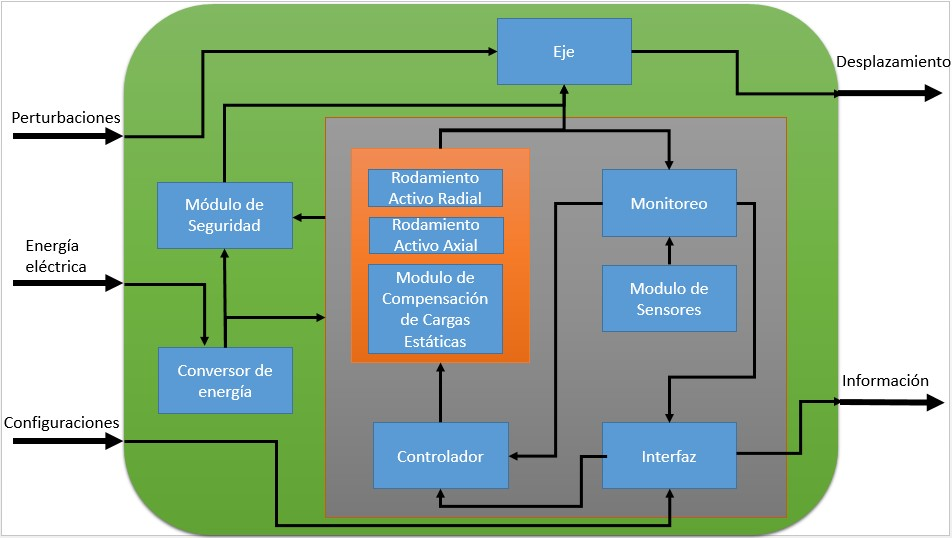
\includegraphics[width=\textwidth]{images/Capitulo_2/DiagramaFuncional}
	\caption{\textit{Diagrama Funcional.}}
	\label{fig:system:example1}
\end{figure}

Del diagrama de �reas funcionales podemos reconocer que el sistema cuenta con 2 entradas que determinan el funcionamiento y el comportamiento del mismo: el suministro de energ�a el�ctrica y las perturbaciones que llegan al sistema. Este diagrama se divide en 3 secciones principales: la primera secci�n lo componen los m�dulos que generan los campos magn�ticos de levitaci�n, los cuales deben variar de acuerdo a lo que indique el controlador. Este se encuentra dominado por el monitoreo del m�dulo de sensores y la interfaz de usuario, la cual adem�s muestra informaci�n sobre la posici�n del rotor. 

La tercera secci�n incluye el convertidor de energ�a que alimenta todos los sistemas el�ctricos, incluyendo el m�dulo de seguridad, el cual se rige a trav�s de la informaci�n que provea el controlador, ya que este s�lo act�a con el corte del suministro el�ctrico o por alguna falla detectada por el controlador. 


\section{Dise�o Conceptual del Producto}

La arquitectura del sistema fue planteada con base en la investigaci�n te�rica sobre las caracter�sticas generales de los rodamientos magn�ticos y en la divisi�n por m�dulos funcionales, de manera que pudieran dise�arse individualmente. 

\subsection{Rodamiento Magn�tico Activo Radial}

Los rodamientos magn�ticos activos utilizan un arreglo de electroimanes opuestos para generar los campos magn�ticos de levitaci�n, y est�n dise�ados para soportar las cargas radiales que act�an sobre el rotor, manteni�ndolo centrado sobre el eje de rotaci�n de la m�quina.

\begin{figure}[htb]
\centering
	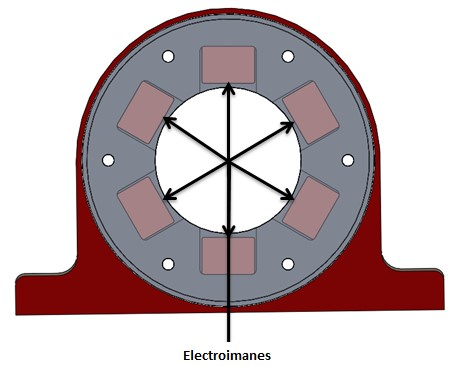
\includegraphics[scale=.65]{images/Capitulo_2/RMAR}
	\caption{\textit{Dise�o conceptual del rodamiento magn�tico activo radial.}}
	\label{fig:system:example1}
\end{figure}

\subsection{Rodamiento Magn�tico Activo Axial}

Como su nombre lo dice, los rodamientos magn�ticos axiales est�n dise�ados para soportar cargas axiales. Estos utilizan un collar de soporte, el cual consiste por lo general en un disco plano, s�lido, de material ferromagn�tico fijado al rotor. Los electroim�nes en forma de disco est�n situados a cada lado del collar y sujetos a la carcasa de la m�quina. Utilizan un sensor o arreglo de sensores que mide la posici�n del rotor en direcci�n axial. 

\begin{figure}[htb]
\centering
	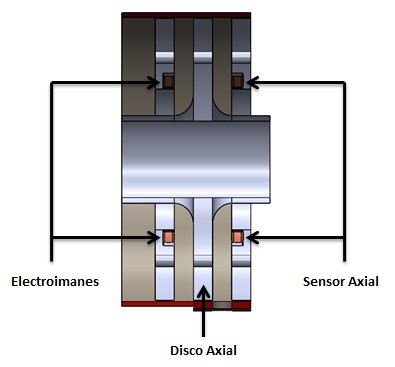
\includegraphics[scale=.65]{images/Capitulo_2/RMAA}
	\caption{\textit{Dise�o conceptual del rodamiento magn�tico activo axial.}}
	\label{fig:system:example1}
\end{figure}

\subsection{M�dulo de Sensores}

Este arreglo de sensores para el rodamiento magn�tico activo radial 
env�a las se�ales de posici�n del rotor al controlador. El controlador utiliza esta informaci�n para modificar el campo electromagn�tico en el rodamiento.

\begin{figure}[htb]
\centering
	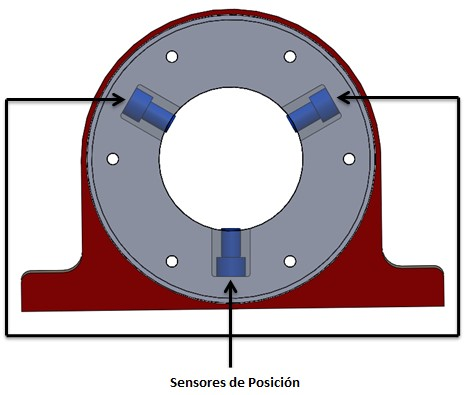
\includegraphics[scale=.65]{images/Capitulo_2/MS}
	\caption{\textit{Dise�o conceptual del arreglo de sensores para los desplazamientos radiales.}}
	\label{fig:system:example1}
\end{figure}

%\clearpage

\subsection{M�dulo de Compensaci�n de Cargas Est�ticas}

Este m�dulo se basa en el principio de funcionamiento de los rodamientos magn�ticos pasivos. Utiliza un im�n permanente para generar un campo magn�tico base de levitaci�n que ayude a disminuir el consumo de energ�a del rodamiento magn�tico radial. Debe utilizar un mecanismo de desplazamiento que var�e la distancia entre el im�n permanente y el rotor para ajustar el campo magn�tico. 

\begin{figure}[htb]
\centering
	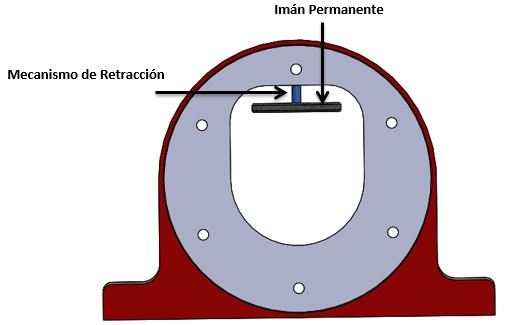
\includegraphics[scale=.70]{images/Capitulo_2/MCCE}
	\caption{\textit{Dise�o Conceptual del m�dulo de compensaci�n para cargas est�ticas.}}
	\label{fig:system:example1}
\end{figure}

\subsection{M�dulo de Seguridad}

Uno de los elementos m�s importantes con los que debe contar un rodamiento magn�tico es un mecanismo auxiliar que tenga como finalidad soportar el rotor en caso de un corte en la energ�a. El rotor no debe de hacer contacto con el mecanismo auxiliar durante el funcionamiento normal de la m�quina.

\begin{figure}[htb]
\centering
	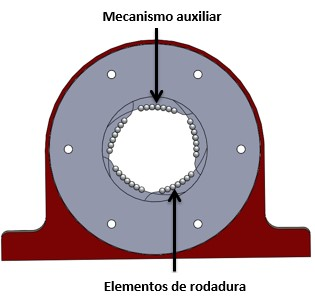
\includegraphics[scale=.90]{images/Capitulo_2/MSG}
	\caption{\textit{Dise�o conceptual del dispositivo auxiliar para el m�dulo de seguridad.}}
	\label{fig:system:example1}
\end{figure}

\subsection{Collar�n de Levitaci�n}

Con el prop�sito de lograr la levitaci�n del rotor sin importar el material del que est� fabricado, se propone el uso de un collar�n de material ferromagn�tico que contenga al eje del rotor dentro del rodamiento. 

\begin{figure}[htb]
\centering
	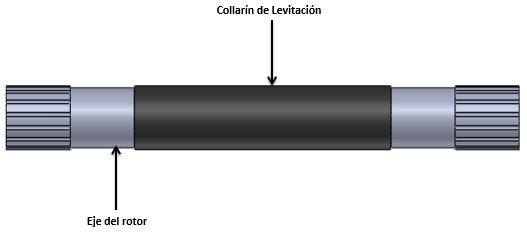
\includegraphics[scale=.90]{images/Capitulo_2/CL}
	\caption{\textit{Dise�o Conceptual del collar�n de levitaci�n.}}
	\label{fig:system:example1}
\end{figure}

\subsection{Rodamiento Magn�tico H�brido: Integraci�n de los M�dulos}

Aunque cada uno de los m�dulos es dise�ado individualmente, est�n contemplados para funcionar de manera conjunta y ser ensamblados dentro del mismo armaz�n. La integraci�n de todos los m�dulos nos dar�a como resultado el Rodamiento Magn�tico H�brido. 

\begin{figure}[htb]
\centering
	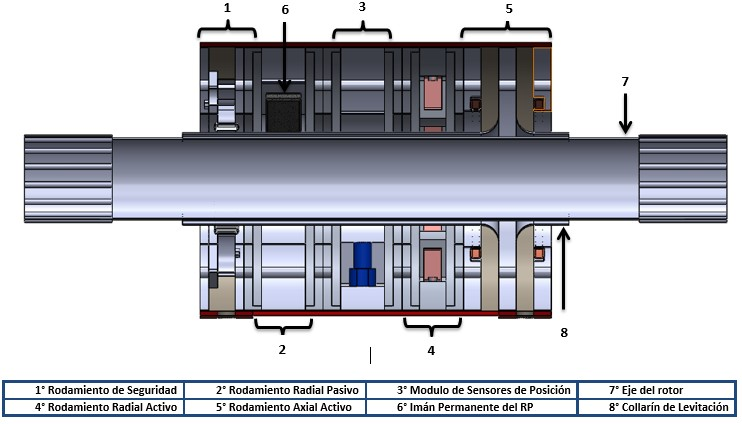
\includegraphics[width=\textwidth]{images/Capitulo_2/RMH}
	\caption{\textit{Dise�o Conceptual del Rodamiento Magn�tico H�brido.}}
	\label{fig:system:example1}
\end{figure}
%%%%%%%%%%%%%%%%%%%%%%%%%%%%%%%%%%%%%%%%%%%%%%%%%%%%%%%%%%%%%%%%%%%
%%%%%%%%%%%%%%%%%%%%%%%%%%%%%%%%%%%%%%%%%%%%%%%%%%%%%%%%%%%%%%%%%%%
\chapter{Dise\~no Detallado}

\section{Dise\~no \'Area Funcional}

C�lculos, Modelos, simulaciones, Selecci�n de componentes, materiales, procesos)

\section{Dise\~no \'Area Funcional n}


\section{Modelo Estructural}\index{Modelado!Modelo Estructural}

El dise�o se hizo con la ayuda de algunas referencias, como una tesis de la Universidad Libre de Berl�n en Alemania, en donde se reporta un proyecto muy parecido al presentado en esta tesis, otras referencias son kits de robots que se venden comercialmente y que presentan algunas de las  caracter�sticas que se plantean en el proyecto.\\

La elecci�n en cuanto al material fue el aluminio, ya que presenta caracter�sticas que  benefician la etapa de construcci�n, por ejemplo: es maleable, f�cil de maquinar, ya sea en un maquinado con arranque de viruta o sin arranque de viruta; su densidad es baja, lo que resulta en un peso bajo, es f�cil de conseguir y relativamente barato.\\


 textte xtetextetetxtetset texttextet extetetxtetset
texttex te textetetxtetset texttextet extet texttextet extetetxtet setet xtetset textte
xtetextetetxtetset texttextet extetetxtetset texttex te textetetxtetset texttextet extet texttextet
extetetxtet setet xtetset




 textte xtetextetetxtetset texttextet extetetxtetset
texttex te textetetxtetset texttextet extet texttextet extetetxtet setet xtetset textte
xtetextetetxtetset texttextet extetetxtetset texttex te textetetxtetset texttextet extet texttextet
extetetxtet setet xtetset


\section{Modelado Matem�tico }\index{Modelado!Modelado Matem�tico}
En el modelo matem�tico se encuentran incluidos todos los factores que intervienen en el comportamiento del robot y dependiendo del tipo de modelado, se puede obtener una simulaci�n del comportamiento real del robot.\\

La cinem�tica estudia el movimiento de alg�n sistema sin tomar en cuenta las fuerzas externas que producen este movimiento o que pudieran afectarlo. En el caso del estudio cinem�tico del robot, se describe su movimiento de manera anal�tica mediante una funci�n que relaciona la posici�n y orientaci�n del punto final del robot con los valores de cada una de las articulaciones del robot. Existen dos tipos de estudios cinem�ticos: Cinem�tica Directa y Cinem�tica Inversa.\\

El problema cinem�tico directo se refiere a expresar la posici�n y orientaci�n del punto final del robot a partir de los valores conocidos de las articulaciones.\\

El problema cinem�tico inverso consiste en conocer los valores que se le deben asignar a cada una de las articulaciones para llegar a la posici�n y orientaci�n deseada.\\

La cinem�tica del robot se representa con la llamada Matriz de Transformaci�n Homog�nea. Esta matriz representa la posici�n y la orientaci�n relativa entre dos eslabones seguidos o unidos. Para trabajar con esta matriz es necesario establecer un sistema de coordenadas. Una herramienta muy utilizada para la descripci�n cinem�tica de robots es el algoritmo de Denavit-Hartenberg (D-H). Con la utilizaci�n de esta herramienta se modela cinem�ticamente el robot. El robot tiene un total de 10 grados de libertad divididos en 5 para cada pierna, sin embargo, las piernas son iguales f�sicamente y su movimiento es similar, as� que en realidad s�lo es necesario modelar una pierna de 5 grados de libertad. \\

Los par�metros a utilizar en el algortimo de D-H se muestran a continuaci�n.\\

\newpage

\begin{figure}[h]
	\centering
		\fbox{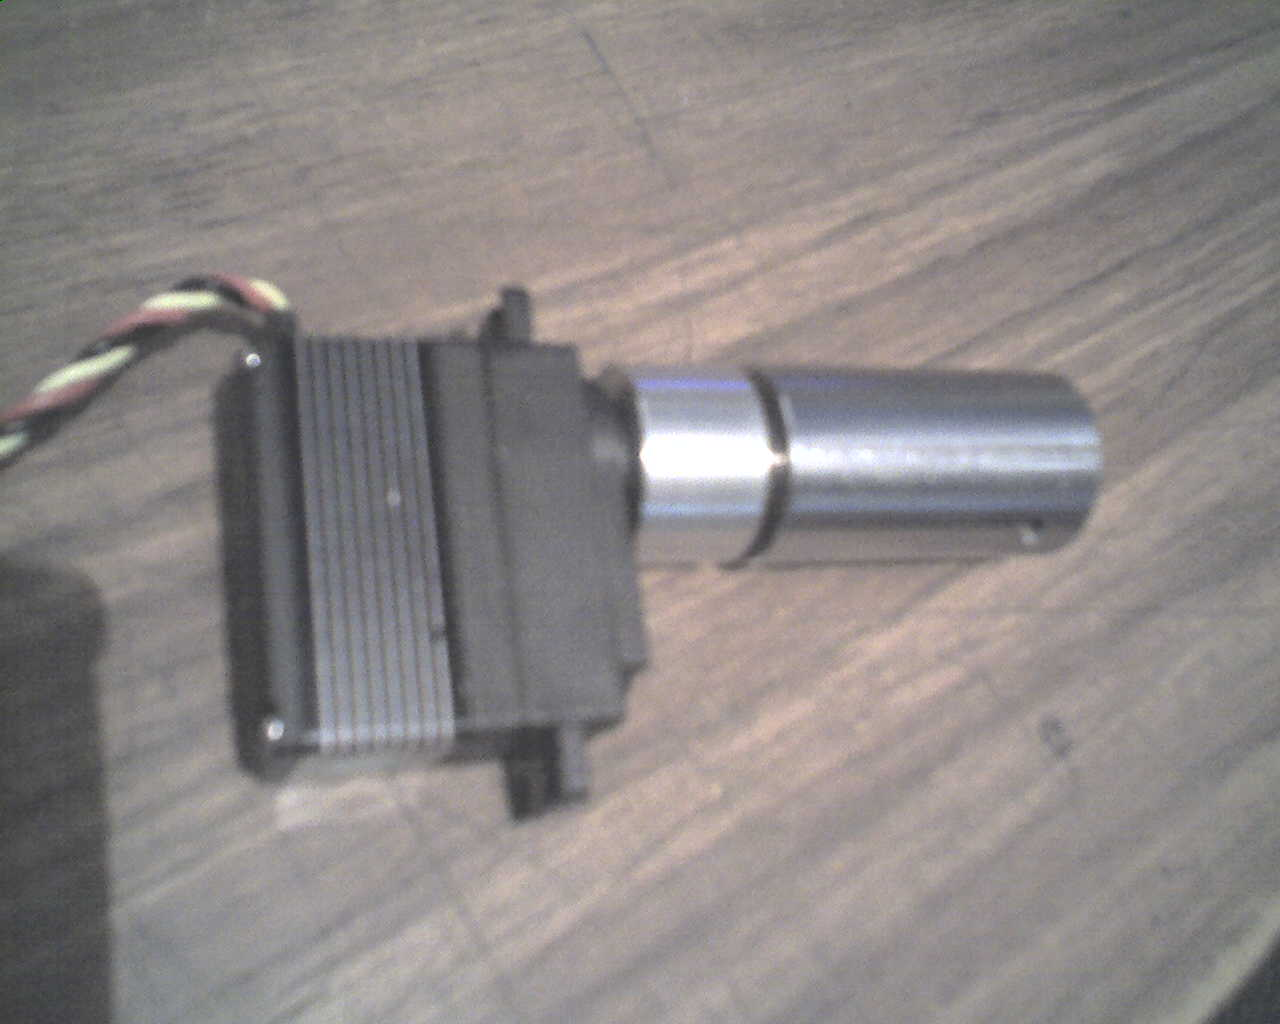
\includegraphics[scale=0.25]{figs/img106.jpg}}
		\caption{Ejes coordenados.}
	\label{fig:DH}
\end{figure}

\begin{table}[h]
	\centering
		\begin{tabular}{|c|c|c|c|c|}
		\hline
			$Eslabon_{i}$	&	$a_{i}$	&	$d_{i}$	&	$\alpha_{i}$ & $\theta_{i}$	\\
			\hline
			0	&	0	&	0	&	0	&	0	\\
			\hline
			1&a1&0&90&q1\\
			\hline
			2&a2&0&0&q2\\
			\hline
			3&a2&0&0&q3\\
			\hline
			4&a1&0&90&q4\\
			\hline
			5&0&0&0&q5\\
			\hline
		\end{tabular}
	\caption{Par�metros de D-H.}
	\label{tab:DH}
\end{table}

Las matrices de transformaci�n Homog�neas obtenidas para cada uno de los eslabones son:\\

\begin{center}

$T_0^1 $= 	\begin{math}
				\left[
				\begin{array}{cccc}
			   	cos(q_1)&               0&         sin(q_1)& 62.82cos(q_1)\\
         sin(q_1)&               0&         cos(q_1)& 62.82sin(q_1)\\
               0&               1&               0&            0 \\
               0&               0&               0&            1

				\end{array}
				\right]
				\end{math}\\
				
\vspace{1cm}

$T_1^2 $= 	\begin{math}
				\left[
				\begin{array}{cccc}
			   	cos(q_2)&	  		 -sin(q_2)&								0&			68.29cos(q_2)\\
          sin(q_2)&          cos(q_2)&                0& 		 68.29sin(q_2)\\
                0&                0&                1&                0\\
                0&                0&                0&                1
				\end{array}
				\right]
				\end{math}\\

\vspace{1cm}				

$T_2^3 $= 	\begin{math}
				\left[
				\begin{array}{cccc}
			   	cos(q_3)&	  		 -sin(q_3)&								0&			68.29cos(q_3)\\
          sin(q_3)&          cos(q_3)&                0& 		 68.29sin(q_3)\\
                0&                0&                1&                0\\
                0&                0&                0&                1

				\end{array}
				\right]
				\end{math}\\
				
\vspace{1cm}				

$T_3^4 $= 	\begin{math}
				\left[
				\begin{array}{cccc}
			   	cos(q_4)&               0&         sin(q_4)& 62.82cos(q_4)\\
         sin(q_4)&               0&         cos(q_4)& 62.82sin(q_4)\\
               0&               1&               0&            0 \\
               0&               0&               0&            1

				\end{array}
				\right]
				\end{math}\\			

\vspace{1cm}

$T_4^5 $= 	\begin{math}
				\left[
				\begin{array}{cccc}
			   	cos(q_5)&	  		 -sin(q_5)&								0&			0)\\
          sin(q_5)&          cos(q_5)&                0& 		 0\\
                0&                0&                1&      0\\
                0&                0&                0&      1

				\end{array}
				\right]
				\end{math}\\
				
				\newpage
				
			
			
{\footnotesize
\begin{center}
				$T_0^5 $= 	
	\begin{math}
\left[
		\begin{array}{ccc}
		\left(\begin{array}{c}
		 cos(q_1)cos(q_5)cos(q_2+q_3+q_4)\\
			   +sin(q_1)sin(q_5)
			   \end{array}\right)&\left(\begin{array}{c}
			   -cos(q_1)sin(q_5)cos(q_2+q_3+q_4)\\
			   +sin(q_1)cos(q_5)
			   \end{array}\right)&cos(q_1)sin(q_2+q_3+q_4\\
			   && \\
\left(\begin{array}{c}
sin(q_1)cos(q_5)cos(q_2+q_3+q_4)\\
-sin(q_1)sin(q_5) \end{array}\right)&\left(\begin{array}{c}
-sin(q_1)sin(q_5)cos(q_2+q_3+q_4)\\
-cos(q_1)cos(q_5)\end{array}\right)&-sin(q_1)sin(q_2+q_3+q_4)\\
   && \\
cos(q_5)sin(q_2+q_3+q_4)&-sin(q_5)sin(q_2+q_3+q_4)&-cos(q_2+q_3+q_4)\\
 & & \\
0&0&0
		\end{array}
				\right]
				\end{math}\\
\end{center}
}
\end{center}

Con este modelo matem�tico es posible generar trayectorias y as� analizar la etapa de caminado. Tambi�n es posible realizar un control de movimiento, sin embargo, este control no ofrecer� la mejor soluci�n, ya que al resolver el problema cinem�tico, no se est�n considerando algunos factores que podr�an afectar al modelo, es por eso que se decide realizar tambi�n un modelado din�mico del sistema.


chos de los sistemas de control que requieren la atenci�n de los
ingenieros son grandes, complejos e involucran muchas variables.
Estos factores est\'an relacionados entre s\'i en modelos
matem\'aticos complicados; las respuestas cuantitativas a estos
problemas se obtienen de soluciones n\'umericas de las ecuaciones
del modelo.

Adem�s de este enfoque para el an\'alisis, es necesario realizar
una investigaci\'on cualitativa simplificada que proporcione
respuestas simples del tipo "si o no'' y que sirvan como una
gu\'ia tanto en el an\'alisis como en el dise\~no.

Las preguntas que se realizan un ingeniero al dise\~nar un sistema
son del tipo: ?`Flotar\'a en barco o se hundir\'a? ?`Se


\section{ Integraci�n}

%%%%%%%%%%%%%%%%%%%%%%%%%%%%%%%%%%%%%%%%%%%%%%%%%%%%%%%%%%%%%%%%%%%
%%%%%%%%%%%%%%%%%%%%%%%%%%%%%%%%%%%%%%%%%%%%%%%%%%%%%%%%%%%%%%%%%%%
%%%%%%%%%%%%%%%%%%%%%%%%%%%%%%%%%%%%%%%%%%%%%%%%%%%%%%%%%%%%%%%%%%%
%%%%%%%%%%%cccccccccc33333333%%%%%%%%%%%%%%%%%%%%%%%%%%%%%%%%%%%%%%
\chapter{Validaci�n y an�lisis de resultados}\index{Validaci�n}

\section{Modelo Estructural}\index{Modelado!Modelo Estructural}

El dise�o se hizo con la ayuda de algunas referencias, como una tesis de la Universidad Libre de Berl�n en Alemania, en donde se reporta un proyecto muy parecido al presentado en esta tesis, otras referencias son kits de robots que se venden comercialmente y que presentan algunas de las  caracter�sticas que se plantean en el proyecto.\\

La elecci�n en cuanto al material fue el aluminio, ya que presenta caracter�sticas que  benefician la etapa de construcci�n, por ejemplo: es maleable, f�cil de maquinar, ya sea en un maquinado con arranque de viruta o sin arranque de viruta; su densidad es baja, lo que resulta en un peso bajo, es f�cil de conseguir y relativamente barato.\\


 textte xtetextetetxtetset texttextet extetetxtetset
texttex te textetetxtetset texttextet extet texttextet extetetxtet setet xtetset textte
xtetextetetxtetset texttextet extetetxtetset texttex te textetetxtetset texttextet extet texttextet
extetetxtet setet xtetset




 textte xtetextetetxtetset texttextet extetetxtetset
texttex te textetetxtetset texttextet extet texttextet extetetxtet setet xtetset textte
xtetextetetxtetset texttextet extetetxtetset texttex te textetetxtetset texttextet extet texttextet
extetetxtet setet xtetset


\section{Modelado Matem�tico }\index{Modelado!Modelado Matem�tico}
En el modelo matem�tico se encuentran incluidos todos los factores que intervienen en el comportamiento del robot y dependiendo del tipo de modelado, se puede obtener una simulaci�n del comportamiento real del robot.\\

La cinem�tica estudia el movimiento de alg�n sistema sin tomar en cuenta las fuerzas externas que producen este movimiento o que pudieran afectarlo. En el caso del estudio cinem�tico del robot, se describe su movimiento de manera anal�tica mediante una funci�n que relaciona la posici�n y orientaci�n del punto final del robot con los valores de cada una de las articulaciones del robot. Existen dos tipos de estudios cinem�ticos: Cinem�tica Directa y Cinem�tica Inversa.\\

El problema cinem�tico directo se refiere a expresar la posici�n y orientaci�n del punto final del robot a partir de los valores conocidos de las articulaciones.\\

El problema cinem�tico inverso consiste en conocer los valores que se le deben asignar a cada una de las articulaciones para llegar a la posici�n y orientaci�n deseada.\\

La cinem�tica del robot se representa con la llamada Matriz de Transformaci�n Homog�nea. Esta matriz representa la posici�n y la orientaci�n relativa entre dos eslabones seguidos o unidos. Para trabajar con esta matriz es necesario establecer un sistema de coordenadas. Una herramienta muy utilizada para la descripci�n cinem�tica de robots es el algoritmo de Denavit-Hartenberg (D-H). Con la utilizaci�n de esta herramienta se modela cinem�ticamente el robot. El robot tiene un total de 10 grados de libertad divididos en 5 para cada pierna, sin embargo, las piernas son iguales f�sicamente y su movimiento es similar, as� que en realidad s�lo es necesario modelar una pierna de 5 grados de libertad. \\

Los par�metros a utilizar en el algortimo de D-H se muestran a continuaci�n.\\

\newpage

\begin{figure}[h]
	\centering
		\fbox{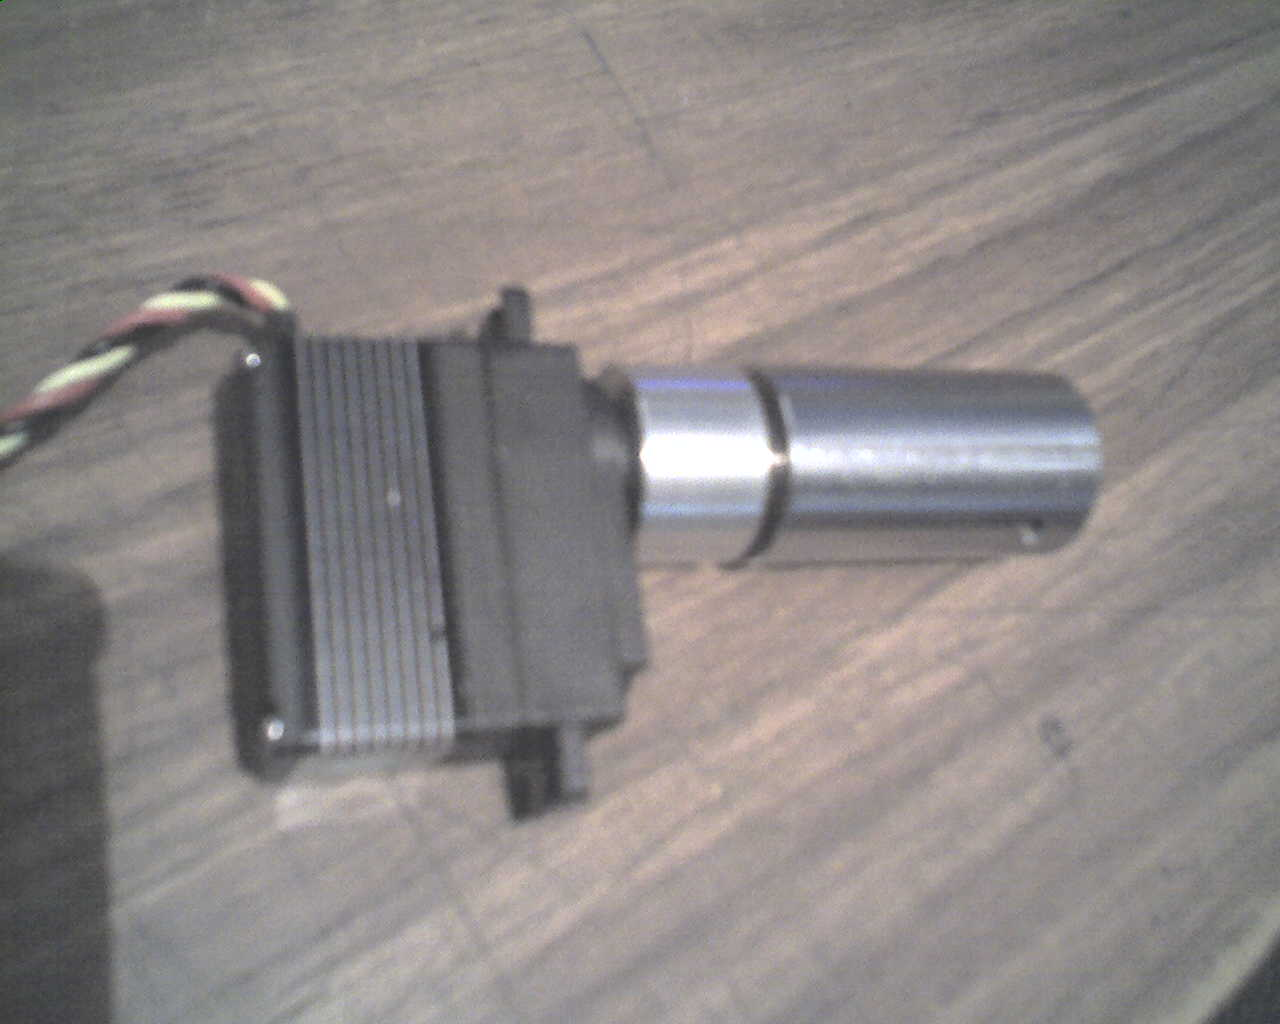
\includegraphics[scale=0.25]{figs/img106.jpg}}
		\caption{Ejes coordenados.}
	\label{fig:DH}
\end{figure}

\begin{table}[h]
	\centering
		\begin{tabular}{|c|c|c|c|c|}
		\hline
			$Eslabon_{i}$	&	$a_{i}$	&	$d_{i}$	&	$\alpha_{i}$ & $\theta_{i}$	\\
			\hline
			0	&	0	&	0	&	0	&	0	\\
			\hline
			1&a1&0&90&q1\\
			\hline
			2&a2&0&0&q2\\
			\hline
			3&a2&0&0&q3\\
			\hline
			4&a1&0&90&q4\\
			\hline
			5&0&0&0&q5\\
			\hline
		\end{tabular}
	\caption{Par�metros de D-H.}
	\label{tab:DH}
\end{table}

Las matrices de transformaci�n Homog�neas obtenidas para cada uno de los eslabones son:\\

\begin{center}

$T_0^1 $= 	\begin{math}
				\left[
				\begin{array}{cccc}
			   	cos(q_1)&               0&         sin(q_1)& 62.82cos(q_1)\\
         sin(q_1)&               0&         cos(q_1)& 62.82sin(q_1)\\
               0&               1&               0&            0 \\
               0&               0&               0&            1

				\end{array}
				\right]
				\end{math}\\
				
\vspace{1cm}

$T_1^2 $= 	\begin{math}
				\left[
				\begin{array}{cccc}
			   	cos(q_2)&	  		 -sin(q_2)&								0&			68.29cos(q_2)\\
          sin(q_2)&          cos(q_2)&                0& 		 68.29sin(q_2)\\
                0&                0&                1&                0\\
                0&                0&                0&                1
				\end{array}
				\right]
				\end{math}\\

\vspace{1cm}				

$T_2^3 $= 	\begin{math}
				\left[
				\begin{array}{cccc}
			   	cos(q_3)&	  		 -sin(q_3)&								0&			68.29cos(q_3)\\
          sin(q_3)&          cos(q_3)&                0& 		 68.29sin(q_3)\\
                0&                0&                1&                0\\
                0&                0&                0&                1

				\end{array}
				\right]
				\end{math}\\
				
\vspace{1cm}				

$T_3^4 $= 	\begin{math}
				\left[
				\begin{array}{cccc}
			   	cos(q_4)&               0&         sin(q_4)& 62.82cos(q_4)\\
         sin(q_4)&               0&         cos(q_4)& 62.82sin(q_4)\\
               0&               1&               0&            0 \\
               0&               0&               0&            1

				\end{array}
				\right]
				\end{math}\\			

\vspace{1cm}

$T_4^5 $= 	\begin{math}
				\left[
				\begin{array}{cccc}
			   	cos(q_5)&	  		 -sin(q_5)&								0&			0)\\
          sin(q_5)&          cos(q_5)&                0& 		 0\\
                0&                0&                1&      0\\
                0&                0&                0&      1

				\end{array}
				\right]
				\end{math}\\
				
				\newpage
				
			
			
{\footnotesize
\begin{center}
				$T_0^5 $= 	
	\begin{math}
\left[
		\begin{array}{ccc}
		\left(\begin{array}{c}
		 cos(q_1)cos(q_5)cos(q_2+q_3+q_4)\\
			   +sin(q_1)sin(q_5)
			   \end{array}\right)&\left(\begin{array}{c}
			   -cos(q_1)sin(q_5)cos(q_2+q_3+q_4)\\
			   +sin(q_1)cos(q_5)
			   \end{array}\right)&cos(q_1)sin(q_2+q_3+q_4\\
			   && \\
\left(\begin{array}{c}
sin(q_1)cos(q_5)cos(q_2+q_3+q_4)\\
-sin(q_1)sin(q_5) \end{array}\right)&\left(\begin{array}{c}
-sin(q_1)sin(q_5)cos(q_2+q_3+q_4)\\
-cos(q_1)cos(q_5)\end{array}\right)&-sin(q_1)sin(q_2+q_3+q_4)\\
   && \\
cos(q_5)sin(q_2+q_3+q_4)&-sin(q_5)sin(q_2+q_3+q_4)&-cos(q_2+q_3+q_4)\\
 & & \\
0&0&0
		\end{array}
				\right]
				\end{math}\\
\end{center}
}
\end{center}

Con este modelo matem�tico es posible generar trayectorias y as� analizar la etapa de caminado. Tambi�n es posible realizar un control de movimiento, sin embargo, este control no ofrecer� la mejor soluci�n, ya que al resolver el problema cinem�tico, no se est�n considerando algunos factores que podr�an afectar al modelo, es por eso que se decide realizar tambi�n un modelado din�mico del sistema.


chos de los sistemas de control que requieren la atenci�n de los
ingenieros son grandes, complejos e involucran muchas variables.
Estos factores est\'an relacionados entre s\'i en modelos
matem\'aticos complicados; las respuestas cuantitativas a estos
problemas se obtienen de soluciones n\'umericas de las ecuaciones
del modelo.

Adem�s de este enfoque para el an\'alisis, es necesario realizar
una investigaci\'on cualitativa simplificada que proporcione
respuestas simples del tipo "si o no'' y que sirvan como una
gu\'ia tanto en el an\'alisis como en el dise\~no.

Las preguntas que se realizan un ingeniero al dise\~nar un sistema
son del tipo: ?`Flotar\'a en barco o se hundir\'a? ?`Se
mantendr\'a en orbita el sat\'elite? ?`? ?`?� ?`
\section{Conceptos b\'asicos}

\section{Criterios de estabilidad}

\subsection{M\'etodo directo de Routh -- Hurwitz}
\subsubsection{M\'etodo de Mikhailov}
\subsubsection{M\'etodo de Hurwitz}
\subsubsection{M\'etodo de Routh}

\subsection{M\'etodo del Lugar de las Ra\'ices}

\subsection{Criterio de Bode}

\subsection{Criterio de Nyquist}
M\'{E}TODO DE NYQUIST PARA EL AN\'{A}LISIS DE ESTABILIDAD DE
SISTEMAS LINEALES

\bigskip

\begin{itemize}
\item  Sistema en lazo cerrado


%\begin{equation*}
%\includegraphics{lc.bmp}
%\end{equation*}

\item  Funci\'{o}n de Tranferencia del sistema en lazo cerrado
\begin{equation*}
\frac{Y(S)}{R(s)}=\frac{G(s)}{1+G(s)H(s)}
\end{equation*}

\item  El sistema en lazo cerrado es estable si todos los polos de la funci\'{o}n de transferencia de lazo cerrado est\'{a}n en el semiplano
izquierdo del plano complejo, es decir,

\begin{quote}
\text{\textit{que ningun polo de lazo cerrado est\'{e} en el}} \\
\text{\textit{semiplano derecho del plano complejo}}
\end{quote}

\newpage

\item  La funci\'{o}n de tranferencia de lazo abierto es $G(s)H(s),$
\end{itemize}

\begin{equation*}
G(s)H(s)=\frac{Z(s)}{P(s)},\qquad Z(s),\text{ }P(s)\text{
}polinomios
\end{equation*}
\quad\ \quad\ *$\quad G(s)H(s)$ es estrictamente propia, o sea, grado de $%
Z(s)<$grado $P(s)$, ello implica
\begin{equation*}
\lim_{\left| s\right| \rightarrow \infty }G(s)H(s)=0
\end{equation*}

\begin{equation*}
1+G(s)H(s)=1+\frac{Z(s)}{P(s)}=\frac{P(s)+Z(s)}{P(s)}
\end{equation*}


\begin{equation*}
\frac{Y(S)}{R(s)}=\frac{G(s)}{1+G(s)H(s)}=\frac{P(s)G(s)}{P(s)+Z(s)}
\end{equation*}

CONCLUSI\'{O}N 1. \ \ Polos de $G(s)H(s)=$ Polos de $1+G(s)H(s)$

CONCLUSI\'{O}N 2. \ Polos de lazo cerado = ceros $1+G(s)H(s)$

\begin{itemize}
\item  CONCLUSI\'{O}N 3. \ De conclusi\'{o}n 2\newline \index{Estabilidad}
``EL sistema es \emph{estable} $\ $\ si \emph{todos los ceros} \ de $%
1+G(s)H(s)$ est\'{a}n en el \emph{semiplano izquierdo} del plano
complejo o \textit{si ninguno de los ceros de }$1+G(s)H(s)$\textit{\
est\'{a} en el semiplano derecho}''\newpage

\item  $1+G(s)H(s)$ como cociente de polinomios
\begin{equation*}
1+G(s)H(s)=k\frac{\left( s+z_{1}\right) \left( s+z_{2}\right) \cdots }{%
\left( s+p_{1}\right) \left( s+p_{2}\right) \left( s+p_{3}\right) \cdots },%
\text{ }k>0
\end{equation*}
\end{itemize}

\^{O}j\^{O} Recordatorio:

$-z_{1,\text{ }}-z_{2,\text{ }}\cdots $, son los polos de lazo
cerrdo,

$-p_{1,\text{ }}-p_{2,\text{ }}\cdots $, son los polos de lazo
abierto, G(s)H(s).



%%%%%%%%%%%%%%%%%%%%%%%%%%%%%%%%%%%%%%%%%%%%%%%%%%%%%%%%%%%%%%%%%%%
%%%%%%%%%%%%%%%%%%%%%%%%%%%%%%%%%%%%%%%%%%%%%%%%%%%%%%%%%%%%%%%%%%%
%%%%%%%%%%%%%%%ccccccccccccccccc44444444444444444%%%%%%%%%%%%%%%%%
%%%%%%%%%%%%%%%%%%%%%%%%%%%%%%%%%%%%%%%%%%%%%%%%%%%%%%%%%%%%%%%%%%%
%%%%%%%%%%%%%%%%%%%%%%%%%%%%%%%%%%%%%%%%%%%%%%%%%%%%%%%%%%%%%%%%%%%
\chapter{Conclusiones}
%%%%%%%%%%%%%%%%%%%%%%%%%%%%%%%%%%%%%%%%%%%%%%%%%%%%%%%%%%%%%%%%%%%%%%%%%%%%%%%%%%%%
\newpage
%%%%%%%%%%%%%%%%%%%%%%%%%%%%%%%%%%%%%%%%%%%%%%%
%%%%%%%%%%%%%%%%%%%%%%%%%%%%%%%%%%%%%%%%%%%%%%%%%%%%%%%%%%%%%%%%%%%%%%%%%%%%%%%%%%%%%%
%%%%%%%%%%%%%%%%%%%%%%%%%%%%%%%  BIBLIOGRAFIA  %%%%%%%%%%%%%%%%%%%%%%%%%%%%%%%%%%%%%%%
%%%%%%%%%%%%%%%%%%%%%%%%%%%%%%%%%%%%%%%%%%%%%%%%%%%%%%%%%%%%%%%%%%%%%%%%%%%%%%%%%%%%%%
\bibliographystyle{plain} \nocite{*}
 \bibliography{xbiblioteca}
%%%%%%%%%%%%%%%%%%%%%%%%%%%%%%%%%%%%%%%%%%%%%%%%%%%%%%%%%%%%%%%%%%%%%%%%%%%%%%%%%
%%%%%%%%%%%%%%%%%%%%%%%%%%%%  INDICE  %%%%%%%%%%%%%%%%%%%%%%%%%%%%%%%%%%%%%%%%%%%%
%%%%%%%%%%%%%%%%%%%%%%%%%%%%%%%%%%%%%%%%%%%%%%%%%%%%%%%%%%%%%%%%%%%%%%%%%%%%%%%%%%
%%%%%%%%%%%%%%%%%%%%%%%%%    APENDICES  %%%%%%%%%%%%%%%%%%%%%%%%%%%%%%%%%%%%
\part{Ap�ndices}
\appendix
\chapter{Der erste Anhang (Ap\'endice)}

Das Appendix (Anhang) Fragment wird einmal an der gew\"{u}nschten Position
im Dokument eingef\"{u}gt. Weitere Anh\"{a}nge k\"{o}nnen dann mittels der
Zuweisung von Abschnitten (sections) erzeugt werden.

\bigskip

Ab hier beginnt der \verb|backmatter|.

\chapter{Der Zweite Anhang (Ap\'endice)}

Das Appendix (Anhang) Fragment wird einmal an der gew\"{u}nschten Position
im Dokument eingef\"{u}gt. Weitere Anh\"{a}nge k\"{o}nnen dann mittels der
Zuweisung von Abschnitten (sections) erzeugt werden.

\bigskip

Ab hier beginnt der \verb|backmatter|.

\chapter{Der Zweite Anhang (Ap\'endice)}

Das Appendix (Anhang) Fragment wird einmal an der gew\"{u}nschten Position
im Dokument eingef\"{u}gt. Weitere Anh\"{a}nge k\"{o}nnen dann mittels der
Zuweisung von Abschnitten (sections) erzeugt werden.

\bigskip

Ab hier beginnt der \verb|backmatter|.

\part{Anexos}
\anexo
\chapter{Hoja de datos)}

Das Appendix (Anhang) Fragment wird einmal an der gew\"{u}nschten Position
im Dokument eingef\"{u}gt. Weitere Anh\"{a}nge k\"{o}nnen dann mittels der
Zuweisung von Abschnitten (sections) erzeugt werden.

\bigskip

Ab hier beginnt der \verb|backmatter|.

\chapter{Der Zweite Anhang (Anexo)}

Das Appendix (Anhang) Fragment wird einmal an der gew\"{u}nschten Position
im Dokument eingef\"{u}gt. Weitere Anh\"{a}nge k\"{o}nnen dann mittels der
Zuweisung von Abschnitten (sections) erzeugt werden.

\bigskip

Ab hier beginnt der \verb|backmatter|.

\chapter{Der Zweite Anhang (Anexo)}

Das Appendix (Anhang) Fragment wird einmal an der gew\"{u}nschten Position
im Dokument eingef\"{u}gt. Weitere Anh\"{a}nge k\"{o}nnen dann mittels der
Zuweisung von Abschnitten (sections) erzeugt werden.

\bigskip

Ab hier beginnt der \verb|backmatter|.

\backmatter
\newpage
\addcontentsline{toc}{chapter}{\'Indice Alfab\'etico}%
\printindex%
\end{document}
%%%%%%%%%%%%%%%%%%%%%%%%%%%%%%%%%%%%%%%%%%%%%%%%%%%%%%%%%%%%%%%%%%%%%%%%%%%%%%%%%% 